\chapter{Описание и валидация бизнес-процесса}

\section{Описание бизнес процесса}

Для начала бегло рассмотрим процесс оказания услуги <<Совет
да любовь>>. Данная услуга оказывается гражданам, прожившим
в браке на территории Свердловской области 50 лет, которые
в силу этого могут быть представлены к награде <<Совет да любовь>>.
Наша услуга подготавливает наградной лист и предложения об
этом достяжении и передает их в правительство.

Начинается все с подачи документов заявителем в многофункциональный
центр, там документы регистрируются и передаются в министерство
Социальной политики Сверловской области (далее, министерство).
Там, если заявителем не были предоставлены сведения о судимости,
отправляется запрос в Информационный центр (ИЦ).
После получения этих сведений, проверяется соблюдения прав
и свобод детей у заявителей. Для этого требуется согласование
с терроториальной комиссией по делам несовершенолетних
и защите их прав (ТКДНиЗП). И согласовав данный этап,
в министерстве оформляется наградной лист и предложения
о награждении, и они передаются в Правительство Свердловской
области.

\clearpage
\section{Создание диаграммы процесса}

Описав кратко моделируемую услугу, перейдем к описанию
этого бизнес-процесса в виде нотации BPMN (Рисунок \ref{description}).

Все элементы процесса размещаются в пуле процесса, который
делится на дорожки, где каждая дорожка представляет исполнителя.
В нашем случе это: заявитель, МФЦ, министерство, ИЦ и ТКДНиЗП.

Бизнес-процесс начинается со стартового события,
зеленого круга (подача заявления), и заканчивается
завершающимся событием, крсным кругом (передача предложений и
наградного листа в Правительство). Между этими событиями
происходит передача управления на выполнение промежуточных
задач, синих прямоугольников.

В добавок к этому, в нашей схеме содержится шлюз, на котором
управление передается в зависимости от того, были
ли в подоваемых документах сведения о судмости заявителей или нет.

Если этих требований не было, то происходит передача сообщений
в информационный центр и обратно. Внутри него данные сведения
могут быть получены разными способами, поэтому данная задача
описана, как комплексная.

\begin{sidewaysfigure}
    \centering
    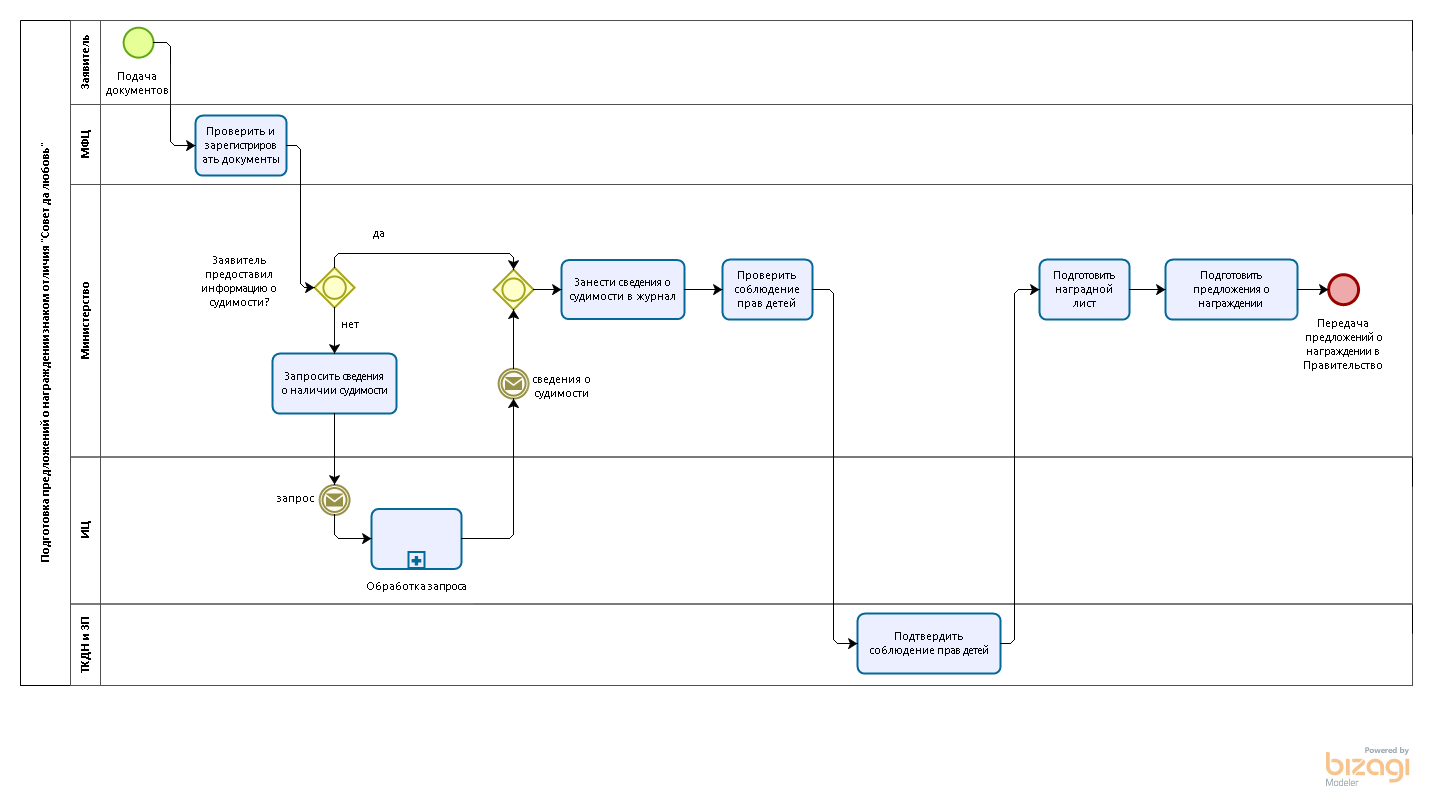
\includegraphics[width=\textwidth]{figures/model-description}
    \caption{Улуга <<Совет да любовь>> в нотации BPMN}
    \label{description}
\end{sidewaysfigure}

\clearpage
\section{Запуск моделирования}


\myImage{}{run_control}{}
\myImage{}{run_if}{}
\myImage{}{run_report}{}